\label{Appendix:ExcelUseage}
\excel\ files are used to store information in the following databases:
\begin{itemize}
  \item \texttt{GWF.xlsx} for \gwf\ domain material parameters.
  \item \texttt{SWF.xlsx} for \swf\ domain material parameters.
  \item \texttt{CLN.xlsx} for \cln\ domain material parameters.
  \item \texttt{SMS.xlsx} for solver parameters.
  \item \texttt{ET.xlsx} and  \texttt{LAI.xlsx} for evapotranspiration (ET) and leaf area index (LAI) parameters respectively.  {\em These are currently just placeholders for future development and will not be discussed further at this time.}
\end{itemize}

Modifications can be made to the database by editing the \texttt{xlsx} file in \excel\ and exporting the results to a \texttt{csv}-formatted version of the file which is then read and processed by \mut.  We will use the \gwf\ database to illustrate the modification workflow, which can then be applied to the other databases.

If you are a \mut\ end-user, you should edit the database files in the \bin\ directory, as outlined on page~\pageref{page:userbin}.

If you are a developer and have downloaded the MUT\_Examples repository, you should edit the database files in the directory \textit{pathto}\texttt{$\backslash$Grdbldr$\backslash$\_MUT\_USERBIN},
where the string \textit{pathto} represents the local path to the repository (e.g.\ \texttt{c:$\backslash$repos}).

First, open the \texttt{GWF.xlsx} in \excel:

    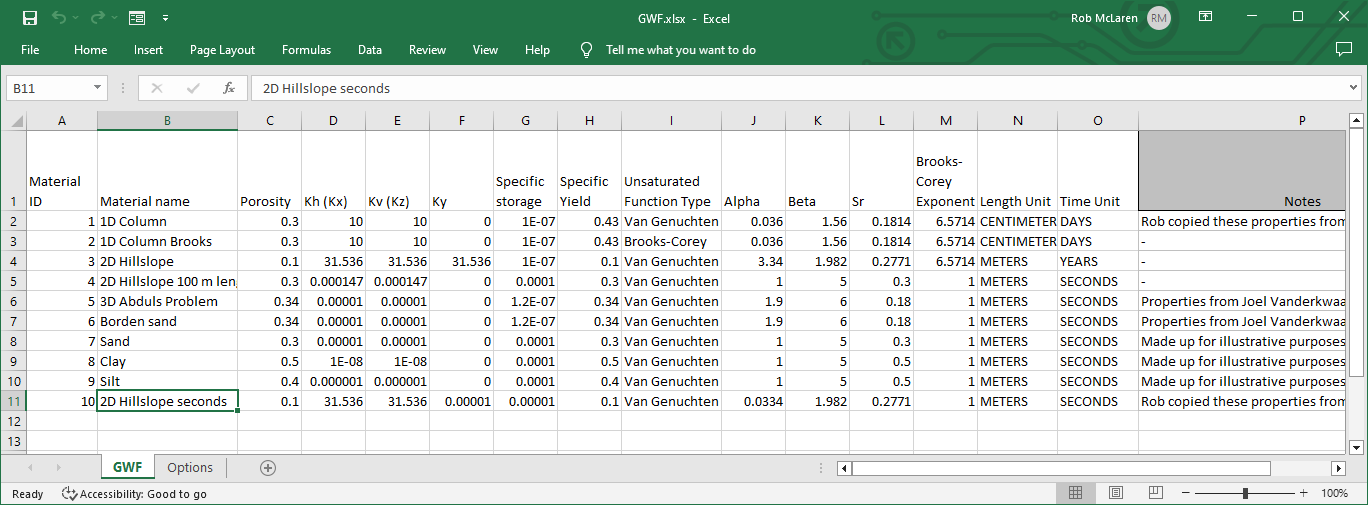
\includegraphics[width=\textwidth]{Excel_1_GWFxlsx}

Some key features to note are:
\begin{itemize}
    \item The first row contains database field (i.e.\ column) names.
    \item The existing database contains data for 10 materials stored in rows 2 to 11.
\end{itemize}

As a precaution, the database is protected. \index{Excel ! cell protection} label If you try to modify any of the existing contents, in this case rows 1 to 11, you will receive the following warning:

    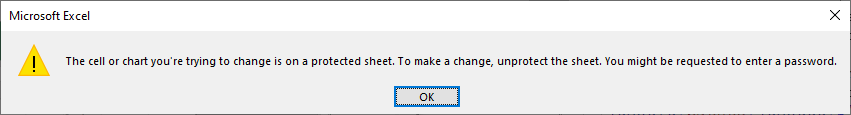
\includegraphics[width=\textwidth]{Excel_2_ProtectionWarning}

To unprotect the sheet, choose {\sf Review}, then {\sf Unprotect sheet}:

   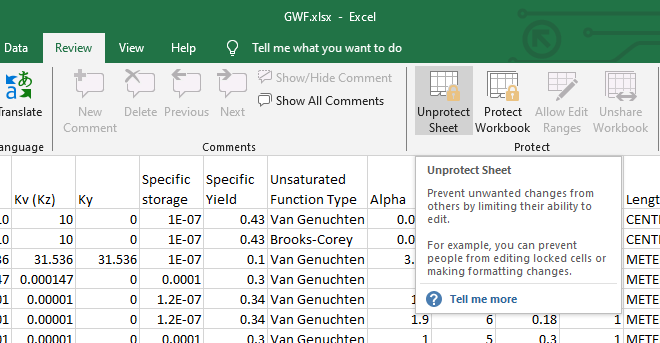
\includegraphics[width=.7\textwidth]{Excel_3_unprotect}

You will be prompted to enter a password, which is {\tt mut}.

To protect the sheet, choose {\sf Review}, then {\sf Protect sheet}, then enter and confirm a password.  We suggest you use the {\tt mut} password.  If not, don't forget the new password!

The purpose for protecting the database is to prevent accidental changes from being made to critical material properties so future runs referring to protected material ID's yield repeatable results.  This would be the case, for example,  for material properties calibrated for an engineering project or verification example, which occupy the first 6 materials in this \gwf\ database).

Although the database is protected, you can add your own materials starting at row 12.  The easiest way to add a material is to copy an existing one.  For example, we can copy row 10 (silt) to row 12:
\begin{enumerate}
    \item Click on the number {\sf 10} at the left end of row 10 to select the entire row.

   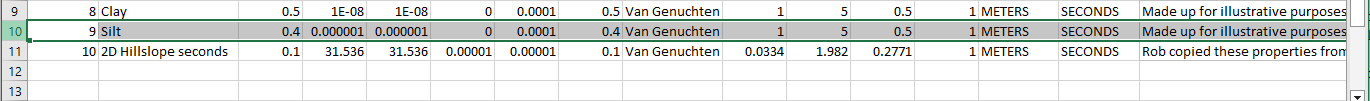
\includegraphics[width=\textwidth]{Excel_4_select}

    \item Type {\tt ctrl-C} to copy it.
    \item Click on the number {\sf 12} at the left end of row 12 to select the entire row.
    \item Type {\tt ctrl-V} to paste it.

   \includegraphics[width=\textwidth]{Excel_5_Paste}

\end{enumerate}
Note that the new material ID number is automatically set to 11, which is the previous number of materials plus 1. You should now change the material name and properties as desired.

If you want to extend the zone of protected cells to include the added row 12 you should do the following:
\begin{enumerate}
    \item Unprotect the worksheet.
    \item Select the entire worksheet by pressing {\tt ctrl-A} or clicking on the 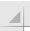
\includegraphics{Excel_SelectAll} button at the top left corner of the worksheet.
    \item {\tt Right-click} on any cell and choose {\sf Format cells...} from the drop-down menu, then in the {\sf Protection} tab uncheck the {\sf Locked} checkbox then choose {\sf OK}.
    
        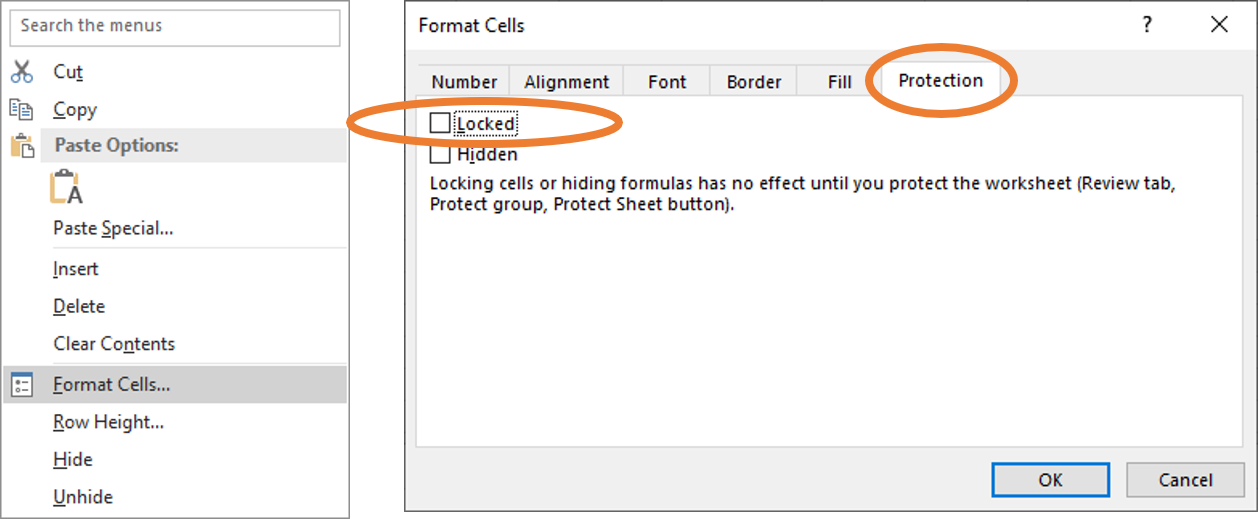
\includegraphics[width=.7\textwidth]{Excel_5b_FormatCells}
    \item Select only the cells containing data that you want to protect, in this case from columns {\sf A} to {\sf P} and rows {\sf 1} to {\sf 12}.
    \item {\tt Right-click} on any chosen cell, choose {\sf Format cells...} from the drop-down menu, then  in the {\sf Protection} tab check the {\sf Locked} checkbox then choose {\sf OK}.
    \item Protect the worksheet.
\end{enumerate}

Columns {\sf I, N} and {\sf O} are special fields where the input is restricted by a list of choices.  For example, if you click on cell {\sf I12}, the {\sf Unsaturated Function Type} for the new material, you will see a drop-down list button 
\includegraphics{Excel_DropListArrow} appear beside the cell.  To choose, for example, the {\sf van Genuchten} function type, select the button and highlight the option in the list and press enter:

   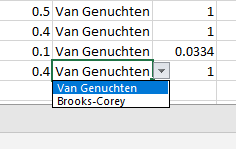
\includegraphics[width=.2\textwidth]{Excel_6_list}

The second worksheet, {\sf Options}, contains the following data:

   \includegraphics[width=.6\textwidth]{Excel_7_Options}

These are the drop-down lists for the unsaturated function type, length unit, time unit in fields I, N and O respectively.  This worksheet is also protected with the password {\tt mut}.

Once you have finished modifying the material properties, you should save the \texttt{xlsx} file, then export them to a \texttt{csv} file by:
\begin{enumerate}
    \item Selecting {\sf File/Export/Change File Type/CSV}:

   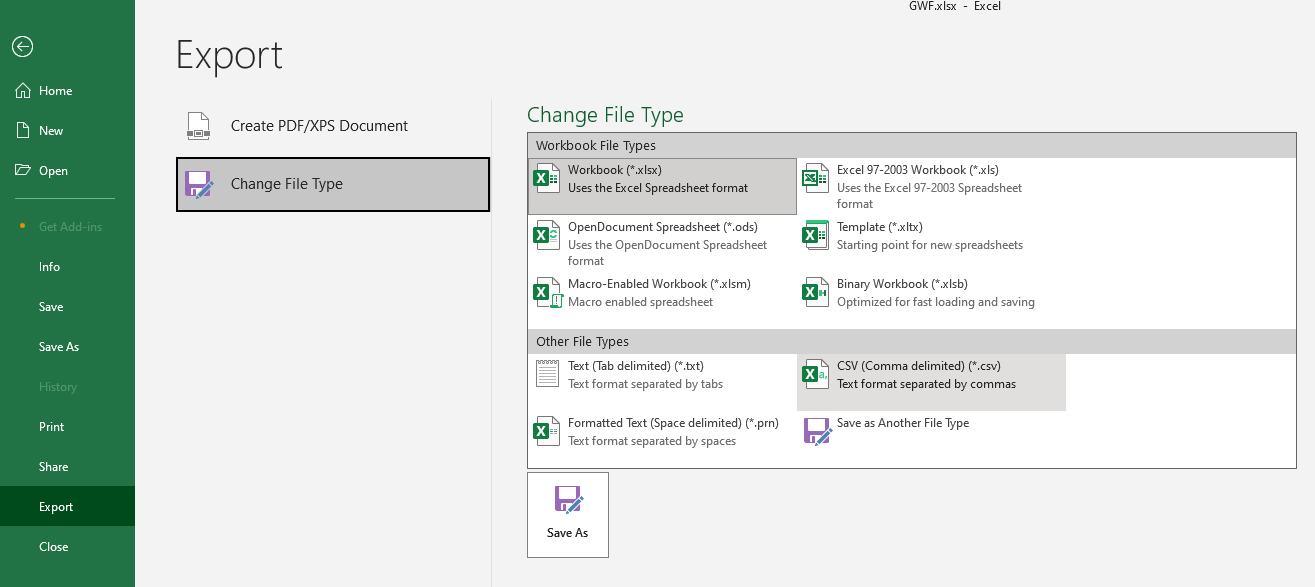
\includegraphics[width=\textwidth]{Excel_8_export}

   \item  Selecting {\sf CSV (Comma delimited)(*.csv)}
   \item  {\tt Clicking} the {\sf Save As} button.
\end{enumerate}





